\documentclass[11pt,a4paper,onecolumn]{article}

% Packages
\usepackage[utf8]{inputenc}
\usepackage[T1]{fontenc}
\usepackage{mathptmx} % Times New Roman font
\usepackage{geometry}
\usepackage{amsmath,amsfonts,amssymb}
\usepackage{graphicx}
\usepackage{fancyhdr}
\usepackage{setspace}
\usepackage{titlesec}
\usepackage[french]{babel}
\usepackage{hyperref}
\usepackage{multicol}

% Page geometry
\geometry{
    left=2.5cm,
    right=2.5cm,
    top=3cm,
    bottom=3cm,
    headheight=14pt
}

% Header and footer
\pagestyle{fancy}
\fancyhf{}
\fancyhead[L]{\leftmark}
\fancyhead[R]{\thepage}
\renewcommand{\headrulewidth}{0.4pt}

% Title formatting
\titleformat{\section}{\Large\bfseries}{\thesection}{1em}{}
\titleformat{\subsection}{\large\bfseries}{\thesubsection}{1em}{}

% Document information
%\title{Document Principal}
%\author{Votre Nom}
%\date{\today}

% Hyperref setup
\hypersetup{
    colorlinks=true,
    linkcolor=black,
    filecolor=magenta,      
    urlcolor=cyan,
    pdftitle={Document Principal},
    pdfpagemode=FullScreen,
}

\begin{document}

% Title page
%\maketitle
%\thispagestyle{empty}

\newpage

% Table des matières
\renewcommand{\contentsname}{Table des matières}
\tableofcontents
\newpage

% Main content
\section{Introduction}
Durant la première séance, nous allons découvrir comment il est possible d’allumer et d’éteindre une LED en réalisant 
un petit montage électronique et en écrivant un script python simple. Cette séance est nécessaire pour comprendre 
quelques bases pour la suite ! \par
Dans la deuxième séance, nous commencerons enfin à utiliser le ruban LED et à le contrôler avec des scripts python toujours
assez simples.
Enfin, dans la dernière séance, nous continuerons notre exploration sur le ruban LED, chacun à son rythme,
on pourra apprendre à créer des effets lumineux plus complexes, et même essayer de les activer via une application téléphone !


% Import sub-parts
\section{\textit{Première Séance}}

\subsection{Le Raspberry Pi 5}
Au cours de nos trois séances, nous allons utiliser un nano-ordinateur (un ordinateur miniature “simplifié”) appelé \textbf{Raspberry Pi 5} (RPi 5), 
qui nous permettra de contrôler une LED simple, ou plusieurs LEDs sur un ruban. Il est d’abord vendu seul, sous forme d’une carte unique 
de la taille d’une carte de crédit, appelée carte mère, mais en fonction du projet à réaliser, il est possible d’ajouter des cartes et des 
composants électroniques complémentaires comme une caméra si on veut filmer, 
des roues pour faire une voiture télécommandée, ou comme dans notre cas un ruban LED !

\begin{figure}[ht]
    \centering
    \includegraphics[width=\textwidth]{./Figures/RPi5_description.png}
    \caption{Le Raspberry Pi 5}
    \label{fig:raspberry_pi_5}
\end{figure}

En général, ces composants supplémentaires se connectent sur les pins (broches) \textbf{GPIO = General Purpose Input/Output}. 
C’est sur ces pins que l’on va connecter nos LEDs; elles permettent au RPi 5 
de communiquer aux LEDs les commandes que nous allons envoyer.

\subsection{Montage électronique}

Pour certains montages électroniques, souvent lorsque l’on est au début d’un projet et que l’on fait ce qu’on appelle du “prototypage”,
on a besoin d’une carte intermédiaire pour connecter les différents composants électroniques, appelée carte à trous. \par
Une carte à trous est une plaque en plastique avec plein de petits trous dans lesquels on peut insérer des fils et des composants électroniques 
(sans avoir besoin de souder). À l’intérieur de la carte à trous, les trous sont connectés entre eux par des bandes métalliques, ce qui permet de
faire des connexions électriques facilement. \par

\begin{figure}[ht]
    \centering
    \includegraphics[width=0.81\textwidth]{./Figures/breadboard.png}
    \caption{Présentation d'une breadboard (carte à trous)}
    \label{fig:breadboard}
\end{figure}

On va connecter la LED à la pin GPIO numéro 16 en suivant le schéma de montage de la figure \ref{fig:led_circuit}.

\begin{figure}[ht]
    \centering
    \includegraphics[width=\textwidth]{./Figures/LED_circuit.png}
    \caption{Montage électronique}
    \label{fig:led_circuit}
\end{figure}

On remarque qu’en plus de la LED (en rouge), il y a une résistance (en beige).
La résistance sert à limiter le courant électrique qui traverse la LED, pour éviter de l’endommager.

\subsection{Analogie électrique}

\subsubsection{Le courant électrique}

Imagine un tuyau rempli d’eau. Chaque goutte d’eau représente un électron. Quand tu ouvres le robinet, les gouttes se déplacent 
d’un bout à l’autre du tuyau.
Dans un circuit électrique, c’est pareil : les électrons (les gouttes d’eau) arrivent par la source d’alimentation et doivent ressortir en 
rejoignant la terre (ou la masse). Augmenter le courant, C’est comme augmenter le débit d’eau dans le tuyau : plus il y a de gouttes (d’électrons) qui circulent par seconde, 
plus le courant est fort.

\subsubsection{La tension électrique}

La tension électrique est comme la pression de l’eau dans le tuyau. Plus la pression est élevée, plus l’eau (ou les électrons)
est poussée avec force à travers le tuyau (ou le circuit). \par
Augmenter la tension, C’est comme monter le tuyau plus haut, au 5ème étage d'un immeuble par exemple : l’eau (les électrons) 
aura plus d’énergie pour circuler, même si le tuyau est un peu plus étroit ou plus long.

\subsection{Programmation Python}

\subsubsection{Démarrage}

Une fois le montage électronique réalisé, on peut brancher le clavier, la souris, et le câble micro-hdmi au Raspberry Pi.
Puis, on peut brancher le câble d'alimentation pour allumer le Raspberry Pi 5.

Il va s'allumer, ou "booter", et afficher l'écran de sélection de l'utilisateur.
On va sélectionner:
\begin{itemize}
    \item Utilisateur : \textbf{illumine}
    \item Mot de passe : \textbf{illumine}
\end{itemize}

Après quelques secondes, le bureau du Raspberry Pi 5 va s'afficher.
On va ouvrir le terminal (icône noire avec un \textgreater\_ blanc) pour pouvoir taper des commandes.

\begin{figure}[ht]
    \centering
    \includegraphics[width=0.8\textwidth]{./Figures/démarrage.png}
    \caption{Bureau du Raspberry Pi 5}
    \label{fig:rpi_desktop}
\end{figure}

\subsubsection{Commandes python}

Pour contrôler la LED, on va utiliser le langage de programmation \textbf{Python}.
Pour comprendre ce qu'est un langage de programmation, on peut faire une analogie 
avec le jeu "Jacques a dit". Dans ce jeu, un joueur donne des instructions aux autres
joueurs, "debout", "saute", "tourne-toi", etc. Les autres joueurs doivent suivre ces instructions.
De la même manière, on va donner des instructions à l'ordinateur, sauf qu'il ne parle pas la même langue
que nous, c'est pour ça qu'on utilise un langage de programmation comme Python. \par

Les premières commandes qu'on va lui donner sont, en français :
\begin{itemize}
    \item "Place toi dans un environnement spécifique"
    \item "Rassemble tes outils"
    \item "Connecte toi à la LED"
    \item "Allume la LED"
    \item "Eteins la LED"
\end{itemize}

En Python, ça donne:
\color{blue}\begin{verbatim}
    cd rpi5_projects/git_repos/illumine/python/1ere_seance/
    source_illumine_env
    ipython
\end{verbatim}

\color{black}
 
Après ces deux premières commandes, on est dans un environnement Python interactif qui ressemble à ça:

\begin{figure}[ht]
    \centering
    \includegraphics[width=0.8\textwidth]{./Figures/ipython.png}
    \caption{Environnement Python interactif}
    \label{fig:ipython}
\end{figure}

On peut maintenant taper les commandes suivantes pour contrôler la LED:
\color{blue}\begin{verbatim}
    from gpiozero import LED
    rouge = LED(16)
    rouge.on()
    rouge.off()
\end{verbatim}

\color{black}

Lance ces commandes une par une dans le terminal en appuyant sur la touche "Entrée" et observe ce qu'il se passe !

\subsubsection{Script python}

On a réussi à allumer et éteindre la LED en tapant les commandes une par une, mais ce n'est pas très pratique.
Si on doit faire ça 10, ou 100 fois, ça va vite devenir lassant. On peut donc automatiser ça en écrivant un script Python,
c'est-à-dire un fichier texte qui contient toutes les commandes à exécuter, et qui est donné en entier à l'ordinateur.
C'est comme une recette de cuisine ! Toutes les étapes sont listées dans l'ordre et l'ordinateur les suit, comme si c'était toi qui
faisait un gâteau. \par

On va d'abord sortir de l'environnement python interactif en faisant \color{blue}\texttt{exit}\color{black}

Toujours dans le terminal, on va ouvrir un éditeur de texte et créer un fichier avec la commande:
\color{blue}\begin{verbatim}
    gedit led_control.py
\end{verbatim}

\color{black}

Une fenêtre va s'ouvrir (patience, ça prend parfois du temps!), c'est l'éditeur de texte. On va écrire les commandes suivantes dans cette fenêtre:
\color{blue}\begin{verbatim}
    from gpiozero import LED
    from time import sleep
\end{verbatim}
\color{black}

Le reste à toi de deviner ! Le but est que la LED s'allume au moins 5 fois. On va utiliser ce qu'on a fait avant, ainsi que
3 commandes données ici dans le désordre:
\color{blue}\begin{verbatim}
    sleep(1)
    print("LED ON")
    print("LED OFF")
\end{verbatim}
\color{black}

Une fois le script terminé, on l'enregistre et on le ferme. Pour le donner à l'ordinateur, c'est-à-dire "l'exécuter", on tape dans le terminal:
\color{blue}\begin{verbatim}
    python3 led_control.py
\end{verbatim}

\color{black}

Essaye d'exécuter ton script plusieurs fois !

\subsubsection{Script avec boucle}

On a vu que le script permet de donner toutes les commandes d'un coup à l'ordinateur, mais on a quand 
même dû écrire toutes les commandes pour allumer et éteindre la LED 5 fois. Si on voulait le faire 100 fois, 
ça ferait beaucoup de lignes à écrire ! Heureusement, en programmation, il existe des structures qui permettent de répéter des actions sans avoir à les écrire plusieurs fois,
ça s'appelle des \textbf{boucles}. \par

On va modifier le script précédent pour utiliser une boucle \textbf{for} qui va répéter l'allumage et l'extinction de la LED 5 fois. 
La structure à utiliser est la suivante:
\color{blue}\begin{verbatim}
    n = #nombre de répétitions
    for i in range(n):
        # instructions à répéter
\end{verbatim}
\color{black}

Essaye de modifier ton script en utilisant cette structure pour allumer et éteindre la LED autant de fois que tu veux !

Une fois le script modifié, enregistre-le et exécute-le à nouveau avec la commande:
\color{blue}\begin{verbatim}
    python3 led_control.py
\end{verbatim}

\color{black}

Amuse-toi à changer le nombre de répétitions et la durée d'allumage/extinction de la LED pour voir ce que ça donne !

\subsubsection{Montage et contrôle de deux LEDs}

Si tu es arrivée jusque là et que tu as envie d'aller plus loin, tu peux refaire
le même montage avec une deuxième LED. Comme tu t'en doutes, on va connecter la deuxième LED
à deux autres pins, les pins 37 et 39 (voir Figure \ref{fig:GPIO}), qui correspondent à la GPIO 26 et à une autre masse (Ground).
Attention aussi à la façon dont tu connectes tes fils à la breadboard !

\begin{figure}[ht]
    \centering
    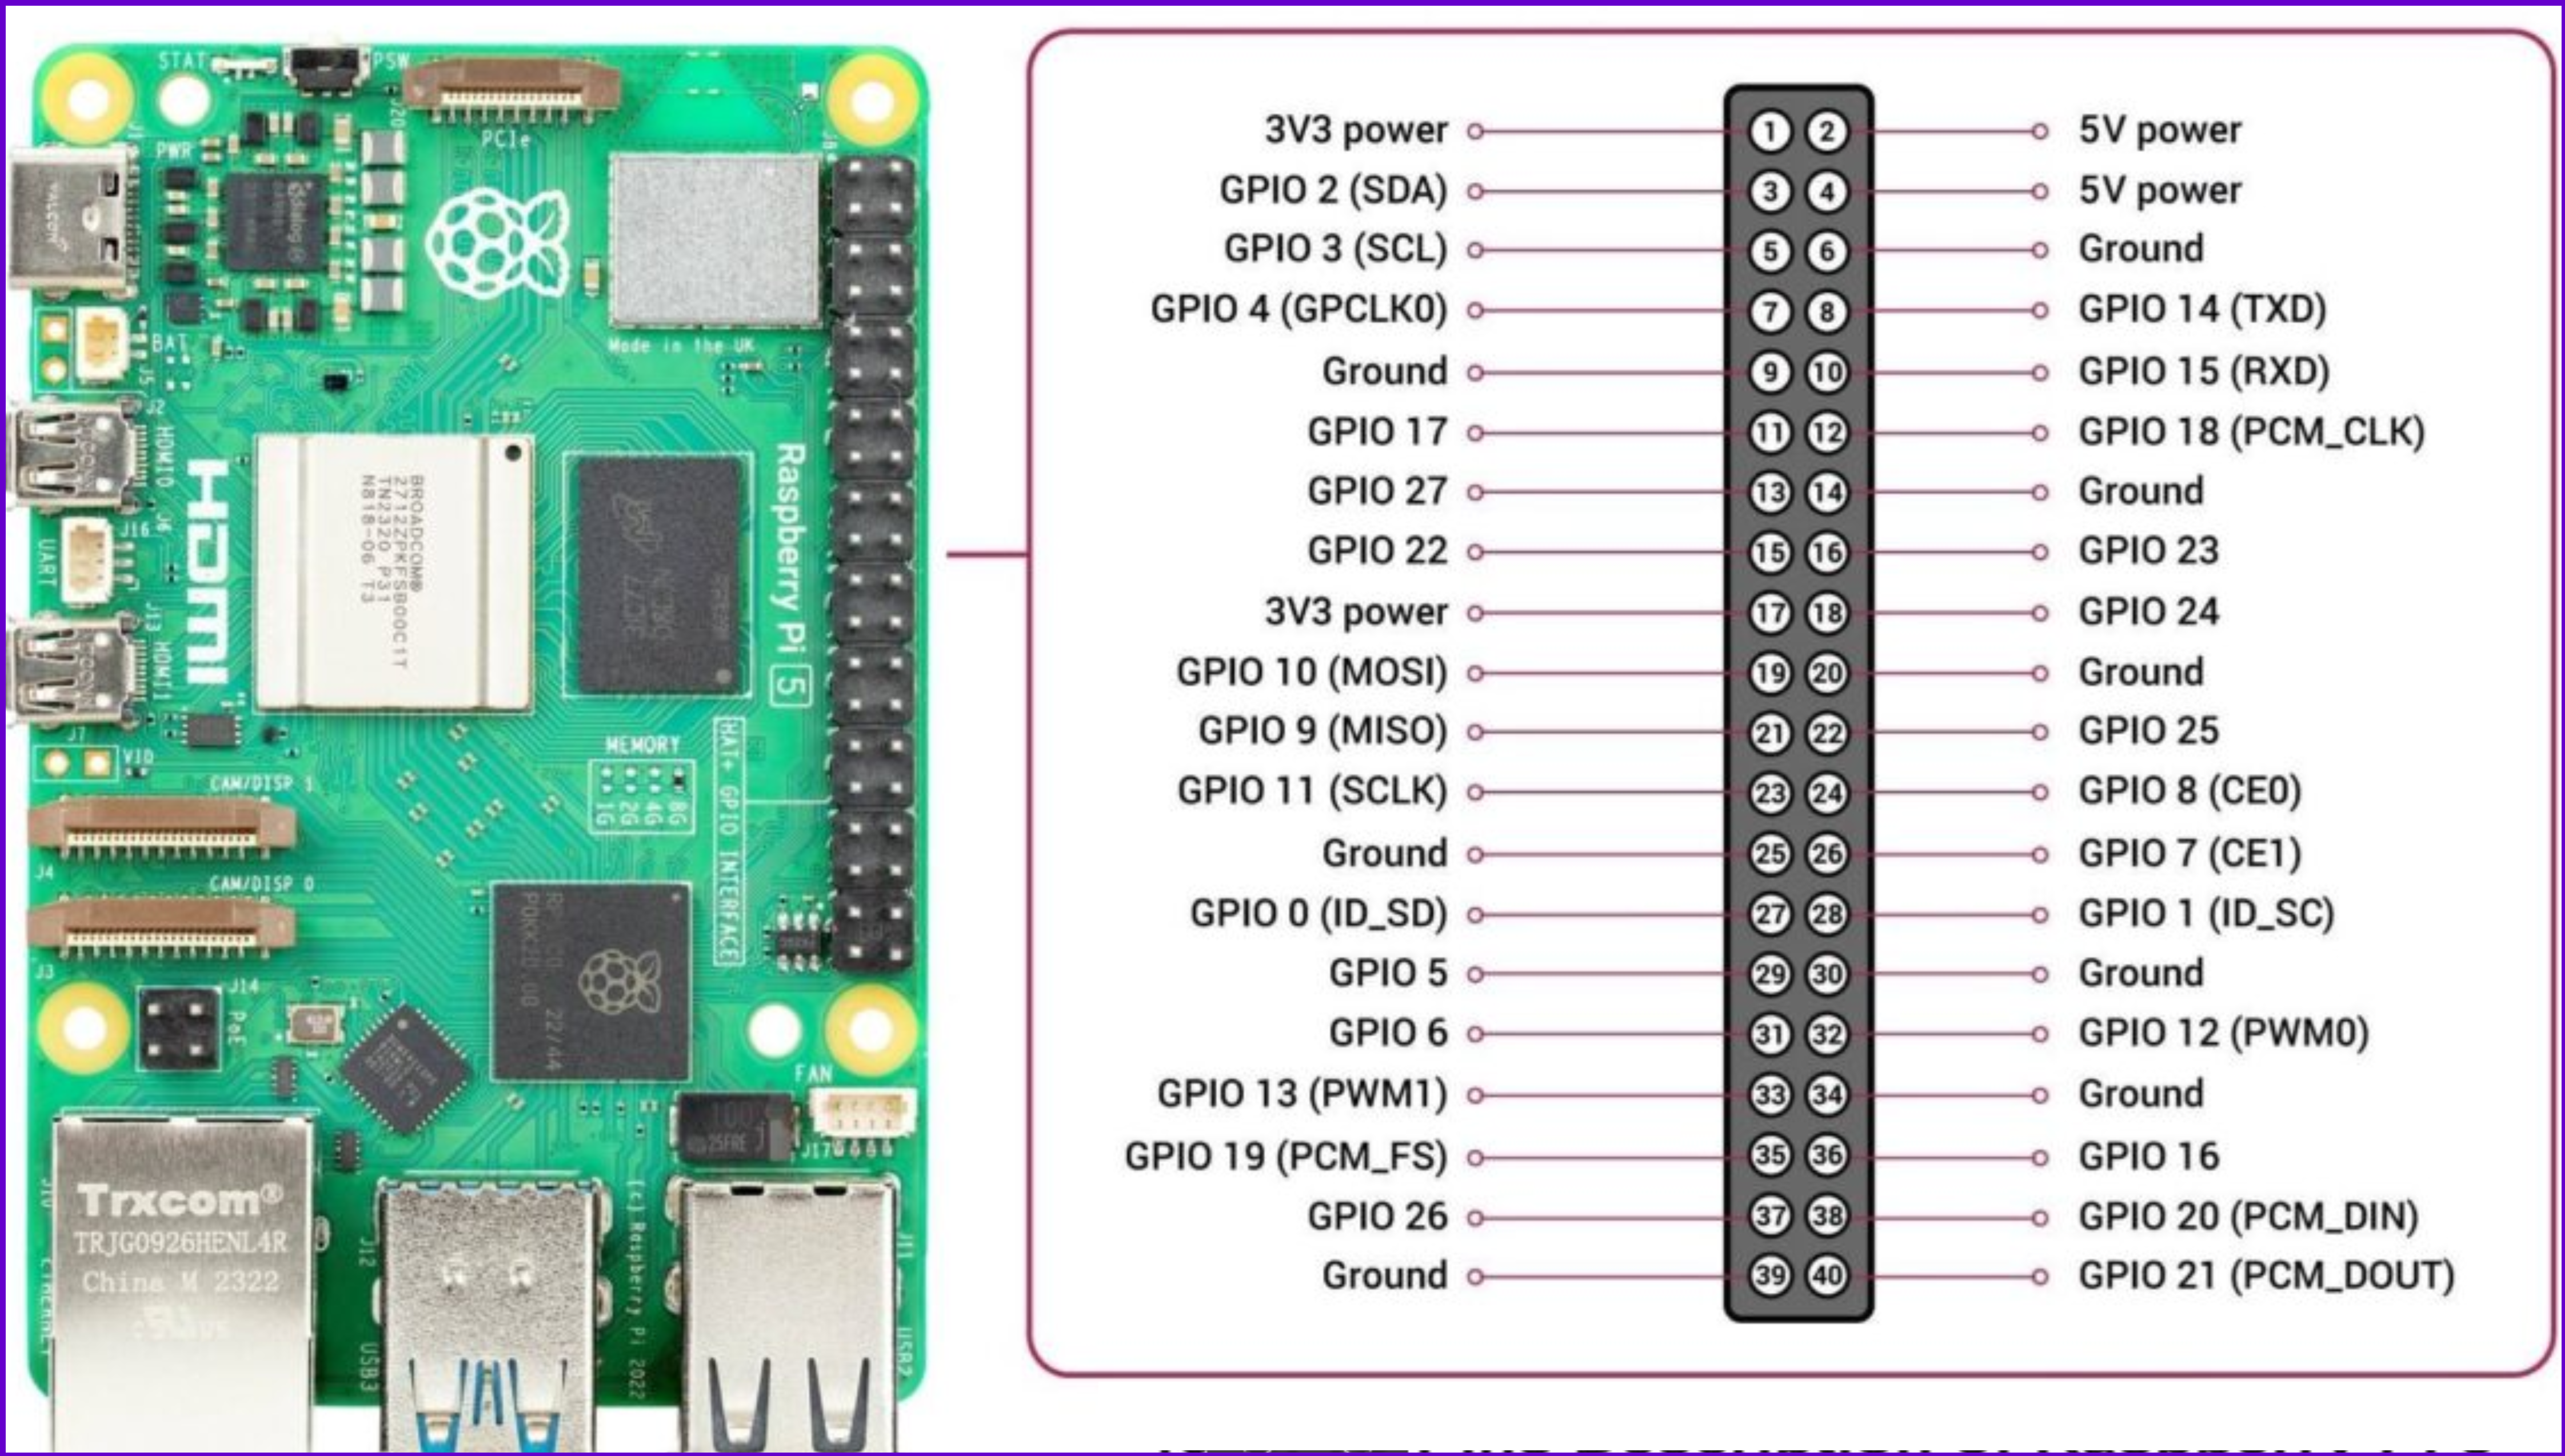
\includegraphics[width=0.9\textwidth]{./Figures/GPIO.png}
    \caption{Liste des GPIOs}
    \label{fig:GPIO}
\end{figure}

Fais vérifier ton montage par un encadrant avant de passer à la suite.

Ensuite, il va falloir modifier ton script Python pour contrôler les deux LEDs. Aide toi de ce que tu as fait avant.
Tu sais maintenant que la pin n'est plus la numéro 16 mais la 26, tu dois donc changer
le numéro quand tu te connectes à la LED. Attention aussi au nom que tu lui donnes,
si tu nommes les deux avec le même nom, l'ordinateur ne saura pas de qui tu parles !

\subsubsection{Eteindre le RPi 5}

On peut éteindre le RPi 5 comme un ordinateur classique, mais on peut aussi l'éteindre avec
une commande dans le terminal:

\color{blue}\begin{verbatim}
    sudo shutdown -h now
\end{verbatim}

\color{black}

Il faut taper le mot de passe: rien ne s'affiche quand tu tapes mais c'est normal !
Tape le bon mot de passe et le RPi 5 va s'éteindre.

Bravo !
\newpage
\section{\textit{Deuxième Séance}}

\subsection{Montage électronique}
On va connecter le ruban LED au raspberry Pi, en utilisant une carte de prototypage, en suivant le schéma ci-dessous:

\begin{figure}[htbp]
    \centering
    \includegraphics[width=\textwidth]{Figures/LED_tape_circuit.png}
    \caption{Schéma de connexion du ruban LED au Raspberry Pi}
    \label{fig:schema_led_tape_rpi}
\end{figure}

\subsection{Programmation Python}

\subsubsection{Démarrage}

Une fois le montage électronique réalisé, on peut brancher le clavier, la souris, et le câble micro-hdmi au Raspberry Pi.
Puis, on peut brancher le câble d'alimentation pour allumer le Raspberry Pi 5.

Il va s'allumer, ou "booter", et afficher l'écran de sélection de l'utilisateur.
On va sélectionner:
\begin{itemize}
    \item Utilisateur : \textbf{illumine}
    \item Mot de passe : \textbf{illumine}
\end{itemize}

Après quelques secondes, le bureau du Raspberry Pi 5 va s'afficher.
On va ouvrir le terminal (icône noire avec un \textgreater\_ blanc) pour pouvoir taper des commandes,
comme montré sur la figure \ref{fig:rpi_desktop}.

\begin{figure}[ht]
    \centering
    \includegraphics[width=0.8\textwidth]{./Figures/démarrage.png}
    \caption{Bureau du Raspberry Pi 5}
    \label{fig:rpi_desktop}
\end{figure}

\subsubsection{Commandes python}

On va se placer dans un environnement python interactif en tapant les commandes suivantes dans le terminal:
\color{blue}\begin{verbatim}
    cd rpi5_projects/git_repos/illumine/python/2eme_seance/
    source_illumine_env
    ipython
\end{verbatim}
\color{black}

On est maintenant dans un environnement Python interactif qui ressemble à celui sur la figure \ref{fig:ipython}.

\begin{figure}[ht]
    \centering
    \includegraphics[width=0.8\textwidth]{./Figures/ipython.png}
    \caption{Environnement Python interactif}
    \label{fig:ipython}
\end{figure}

On peut donc taper des commandes python pour contôler le ruban LED:
\color{blue}\begin{verbatim}
    import RPi5_Neopixel as np 
    ruban = np.Neopixel_Tape()
    ruban.on_all_led('orchid')
\end{verbatim}
\color{black}

On remarque qu'il faut donner un nom de couleur en anglais, alors voici la liste des couleurs disponibles:

\color{blue}
\begin{multicols}{3}
\begin{verbatim}
    'red'
    'dark_red'
    'red_orange'
    'crimson'
    'rust'
    'blood_red'
    'tomato'
    'reddish_orange'
    'burnt_orange'
    'pumpkin'
    'orange'
    'dark_orange'
    'golden_orange'
    'yellow_orange'
    'yellow'
    'bright_yellow'
    'lemon_yellow'
    'pale_yellow'
    'lime_yellow'
    'chartreuse'
    'spring_green'
    'light_green'
    'green'
    'dark_green'
    'forest_green'
    'teal_green'
    'teal'
    'bright_turquoise'
    'medium_turquoise'
    'dark_turquoise'
    'cyan'
    'light_cyan'
    'aqua'
    'light_sky_blue'
    'cornflower_blue'
    'steel_blue'
    'dodger_blue'
    'light_blue'
    'powder_blue'
    'cadet_blue'
    'lavender_blue'
    'light_indigo'
    'indigo'
    'blue_violet'
    'purple'
    'medium_purple'
    'orchid'
    'violet'
    'thistle_purple'
    'pink_purple'
    'magenta'
    'fuchsia'
    'hot_pink'
    'light_pink'
    'pink'
    'light_coral'
    'salmon_pink'
    'coral'
    'tomato_pink'
    'rosy_brown'
\end{verbatim}
\end{multicols}
\color{black}

N'oublie pas les guillements autour du nom de la couleur !

\subsubsection{Fonctions élémentaires}

Plusieurs fonctions élémentaires sont disponibles pour piloter une ou plusieurs LED du ruban. \par

\textit{Exercice:} Essaye les fonctions suivantes en remplaçant \textbf{num} par un numéro de LED entre 0 et 59,
\textbf{color\_name} par un nom de couleur de la liste précédente, et \textbf{times} par le nombre de fois
que tu veux faire l'effet.
Décris sur les pointillés ce que fait chaque fonction.

\color{blue}\begin{verbatim}
    ruban.on_led(num, color_name): ............................................... 

    ruban.off_led(num): ..........................................................

    ruban.on_all_led(color_name): ................................................

    ruban.off_all_led(): .........................................................

    ruban.avance(num, color_name, times): ........................................

    ruban.recule(num, color_name, times): ........................................

    ruban.clignote(num, color_name, times): ......................................

    ruban.clignote_all(color_name, times): .......................................

    ruban.random(color_name, times): ............................................

    ruban.fill_rainbow(): ........................................................
\end{verbatim}
\color{black}

\subsubsection{Script python}

Nous allons maintenant écrire des fonctions plus complexes, mais pour cela nous devons rapidement expliquer
ce que fait une boucle \textit{while}.
Une boucle \textit{while} permet de répéter une série d'instructions tant qu'une condition est vraie.
Une analogie peut être "tant que je ne suis pas arrivée au bout du chemin, je continue d'avancer".
Voici un exemple de boucle \textit{while} en python (à ne pas taper, c'est juste un exemple):
\color{blue}
\begin{verbatim}
    compteur = 0
    while compteur < 5:
        compteur = compteur + 1
\end{verbatim}
\color{black}

On va maintenant quitter l'environnement python interactif en tapant la commande \color{blue}
\texttt{exit()} \color{black}.

\textit{Exercice:} Tape la commande suivante pour ouvrir et compléter le script python \texttt{charge.py}:
\color{blue}
\begin{verbatim}
    gedit charge.py
\end{verbatim}
\color{black}

Une fenêtre comme celle de la figure \ref{fig:charge} va s'ouvrir. La description de la fonction est donnée, 
et c'est à toi de compléter le script en utilisant les fonctions élémentaires vues précédemment, ainsi qu'une
ou plusieurs boucles \textit{while} si nécessaire (et/ou \textit{for}).

\begin{figure}[ht]
    \centering
    \includegraphics[width=0.8\textwidth]{./Figures/fonction_à_compléter.png}
    \caption{Fonction \texttt{charge.py} à compléter}
    \label{fig:charge}
\end{figure}

Une fois terminé, sauvegarde le fichier (Ctrl+S), et tu peux soit fermer la fenêtre et revenir au terminal, soit
garder la fenêtre ouverte, ouvrir un autre terminal et retaper:
\color{blue} 
\begin{verbatim} 
    cd rpi5_projects/git_repos/illumine_ton_ingeniosite/2nd_seance/
    source_illumine_env
\end{verbatim}
\color{black} 

Dans les deux cas, tape:
\color{blue}
\begin{verbatim}
    python3 charge.py
\end{verbatim}
\color{black}
pour exécuter ton script python et voir si le résultat est celui attendu !

Refait cela en remplaçant la fonction \texttt{charge.py} par les fonctions \texttt{chariot.py}
et \texttt{croise.py}.

\subsubsection{Eteindre le RPi 5}

On peut éteindre le RPi 5 comme un ordinateur classique, mais on peut aussi l'éteindre avec
une commande dans le terminal:

\color{blue}\begin{verbatim}
    sudo shutdown -h now
\end{verbatim}

\color{black}

Il faut taper le mot de passe: rien ne s'affiche quand tu tapes mais c'est normal !
Tape le bon mot de passe et le RPi 5 va s'éteindre.

Bravo !




\section{Troisième Partie}

A venir...
\newpage
\section{\textit{Annexe à destination des encadrants}}

\subsection{Matériel}
\label{sec:matériel}

Voici la liste du matériel utilisé pour ce TP. Des produits similaires peuvent
être utilisés, vous pouvez vous référer à la section \ref{sec:références} pour
comprendre les spécificités du matériel.

\begin{itemize}
    \item \textbf{Raspberry Pi 5} 4 Go BCM2712 2,4 GHz \url{https://fr.rs-online.com/web/p/raspberry-pi/0219253}
    \item \textbf{Carte mémoire} A2 class micro-SD cards for DDR50 and SDR104 32GB  \url{https://mou.sr/3Km0bGc} 
    \item \textbf{Alimentation pour Raspberry Pi} 1.2m USB type C avec Fiche femelle européenne \url{https://fr.rs-online.com/web/p/alimentations-raspberry-pi/0219261}
    \item \textbf{Adafruit NeoPixel} Digital RGBW LED Strip - White PCB 60 LED/m 1m \url{https://mou.sr/40tlNWa} 
    \item \textbf{Female DC Power Adapter} \url{https://mou.sr/3NrRk6Y}
    \item \textbf{Adaptateur AC/DC} 5V c.c., 4A, 24W, C14 \url{https://fr.rs-online.com/web/p/adaptateurs-ac-dc/9048474} 
    \item \textbf{Cordon d'alimentation RS PRO} Connecteur CEI C13 CEE 7/7, 1m, 10 A / 250 V \url{https://fr.rs-online.com/web/p/cordons-d-alimentation/6266751} 
    \item \textbf{TXB0104 Bi-Direction Level Shifter} \url{https://mou.sr/4heobXq} 
    \item \textbf{HDMI vers micro HDMI} 1 m \url{https://fr.rs-online.com/web/p/cables-raspberry-pi/2012171} 
    \item \textbf{Platine d'essai} \url{https://fr.rs-online.com/web/p/platines-d-essais/2153175}
    \item \textbf{Strap pour platine d'essai mâle-mâle} \url{https://fr.rs-online.com/web/p/straps-pour-platines-d-essai/2048241}
    \item \textbf{Strap pour platine d'essai mâle-femelle} \url{https://fr.rs-online.com/web/p/straps-pour-platines-d-essai/2048243}
\end{itemize}

Si vous souhaitez réaliser la première séance avec une LED unique, il en faudra également une,
ainsi qu'une résistance. \par
\textit{\textbf{Note:}} Si vous utilisé le convertisseur de niveau (Level-Shifter) proposé ici, il faudra souder
les broches fournies avec vous même. 

\subsection{Configuration du Raspberry Pi}

Dans un premier temps, il faut installer Raspberry Pi OS sur la carte mémoire et configurer le Raspberry Pi 5. Pour simplifier cette étape,
vous trouverez dans ce Proton Drive une image de la carte mémoire déjà configurée.

\textit{\textbf{Lien vers l'image de la carte mémoire:}} \url{https://drive.proton.me/urls/3HZFCYNRZ4#hk5mEik54Qc6}

L'environnement virtuel  python \color{blue} \texttt{illumine\_env} \color{black} est déjà créé et contient toutes les librairies nécessaires, mais voici 
la liste de celles assez spécifiques si vous souhaitez le refaire vous même:
\begin{itemize} \color{blue}
    \item gpiozero
    \item Adafruit-Blinka-Raspberry-Pi5-Neopixel
    \item adafruit-circuitpython-pixelbuf
    \item adafruit-circuitpython-led-animation
    \item ipython
\end{itemize} \color{black}
En plus, vous aurez besoin de librairies plus classiques comme \color{blue}\texttt{numpy}, \texttt{time} \color{black}, etc.

\textit{\textbf{Note:}} Si vous modifiez les chemins des dossiers, n'oubliez pas de modifier le TP en conséquence (commande \color{blue} \texttt{cd} \color{black}).

\subsection{Références et ressources}
\label{sec:références}

Toutes les explications claires et détaillées sont disponibles sur le merveilleux site d'Adafruit.
\begin{itemize}
    \item Une présentation des rubans LED NeoPixel: \url{https://learn.adafruit.com/neopixels-on-raspberry-pi}
    \item Comment réaliser le montage électronique: \url{https://learn.adafruit.com/neopixels-on-raspberry-pi/raspberry-pi-wiring} 
    \item Les librairies python à installer et un exemple de code: \url{https://learn.adafruit.com/neopixels-on-raspberry-pi/python-usage}
    \item Les modifications nécessaires pour le Raspberry Pi 5: \url{https://learn.adafruit.com/circuitpython-on-raspberrypi-linux/using-neopixels-on-the-pi-5}
    \item Présentation du Level Shifter TXB0104: \url{https://www.adafruit.com/product/1875}
\end{itemize}

Si vous souhaitez réaliser le première séance avec une LED unique, voici des ressources utiles:
\begin{itemize}
    \item Le circuit électronique simple \url{https://raspberry-pi.fr/led-raspberry-pi/}
    \item La librairie gpiozero \url{https://raspberrypi.stackexchange.com/questions/148686/raspberry-pi-5-gpiozero}
\end{itemize}

%\section{Conclusion}

\end{document}
